\part{Arduino}
\chapter{Hardware}
\section{Beskrivelse}
Dette er en udviklingsplatform med både WiFi og Bluetooth, baseret på ESP32-chippen, som er integreret med ESP32-WROOOM-32-modulet og er kompatibel med Arduino. Platformen inkluderer en hall-sensor, højhastigheds SDIO/SPI, UART, I2S og I2C-grænseflader. Den er også udstyret med freeRTOS-operativsystemet, hvilket gør den særligt velegnet til projekter inden for Internet of Things (IoT) og smarthjem-teknologi.

\section{Specification}
\begin{itemize}
	\item Spænding: 3,3V-5V
	\item Strømudgang: 1,2A (maksimalt)
	\item Maksimal effektudgang: 10W
	\item Arbejdstemperatur: -10℃~50℃
	\item Dimensioner: 69*54*14,5mm
	\item Vægt: 25,5g
	\item Miljøbeskyttelsesegenskaber: ROHS
\end{itemize}
\clearpage
\section{EPS32 Plus Pins}
\begin{figure}[!h]
	\centering
	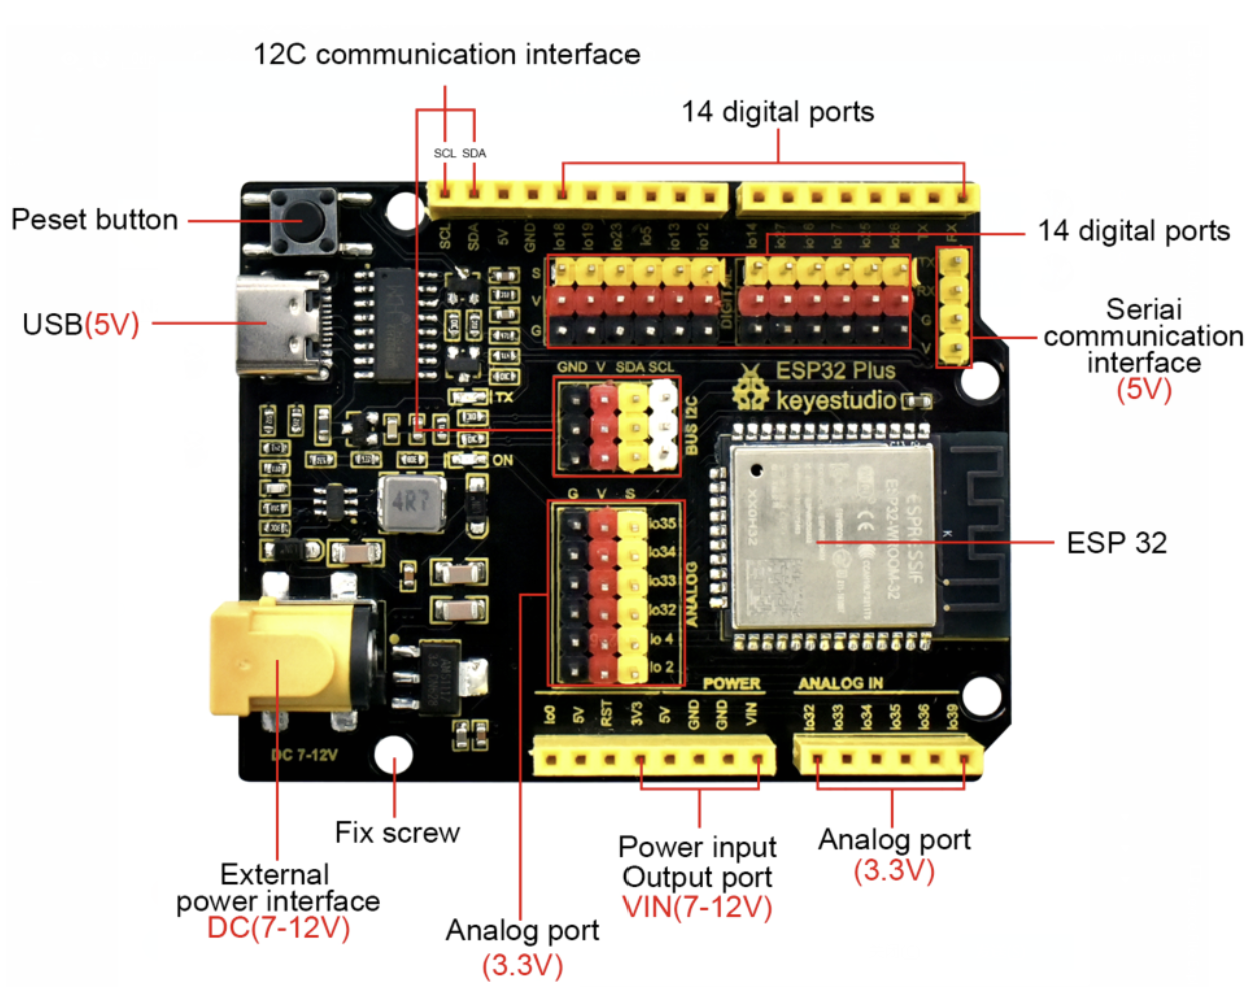
\includegraphics[width=\textwidth]{fig/fig22.png}
	\caption{ESP32 Plus pins}
\end{figure}
\clearpage
\section{Arduino IDE}
\subsection{Introduktion}
Arduino IDE er et open-source værktøj, der bruges til at skrive og uploade kode til Arduino boards. Det understøtter mange forskellige Arduino boards og tilbyder en brugervenlig grænseflade til udvikling af embedded systemer.

\subsection{Installationstrin}
\begin{enumerate}
	\item Start med at downloade \textbf{Arduino IDE} fra \url{https://www.arduino.cc/en/software}. Vælg den version, der passer til dit operativsystem (Windows, macOS eller Linux).
	\item Følg installationsvejledningen på Arduino websitet for at installere Arduino IDE på din computer.
	\item Efter installationen, åbn Arduino IDE. Du skulle nu se en simpel teksteditor med flere funktioner og værktøjslinjer.
	\begin{figure}[!h]
		\centering
		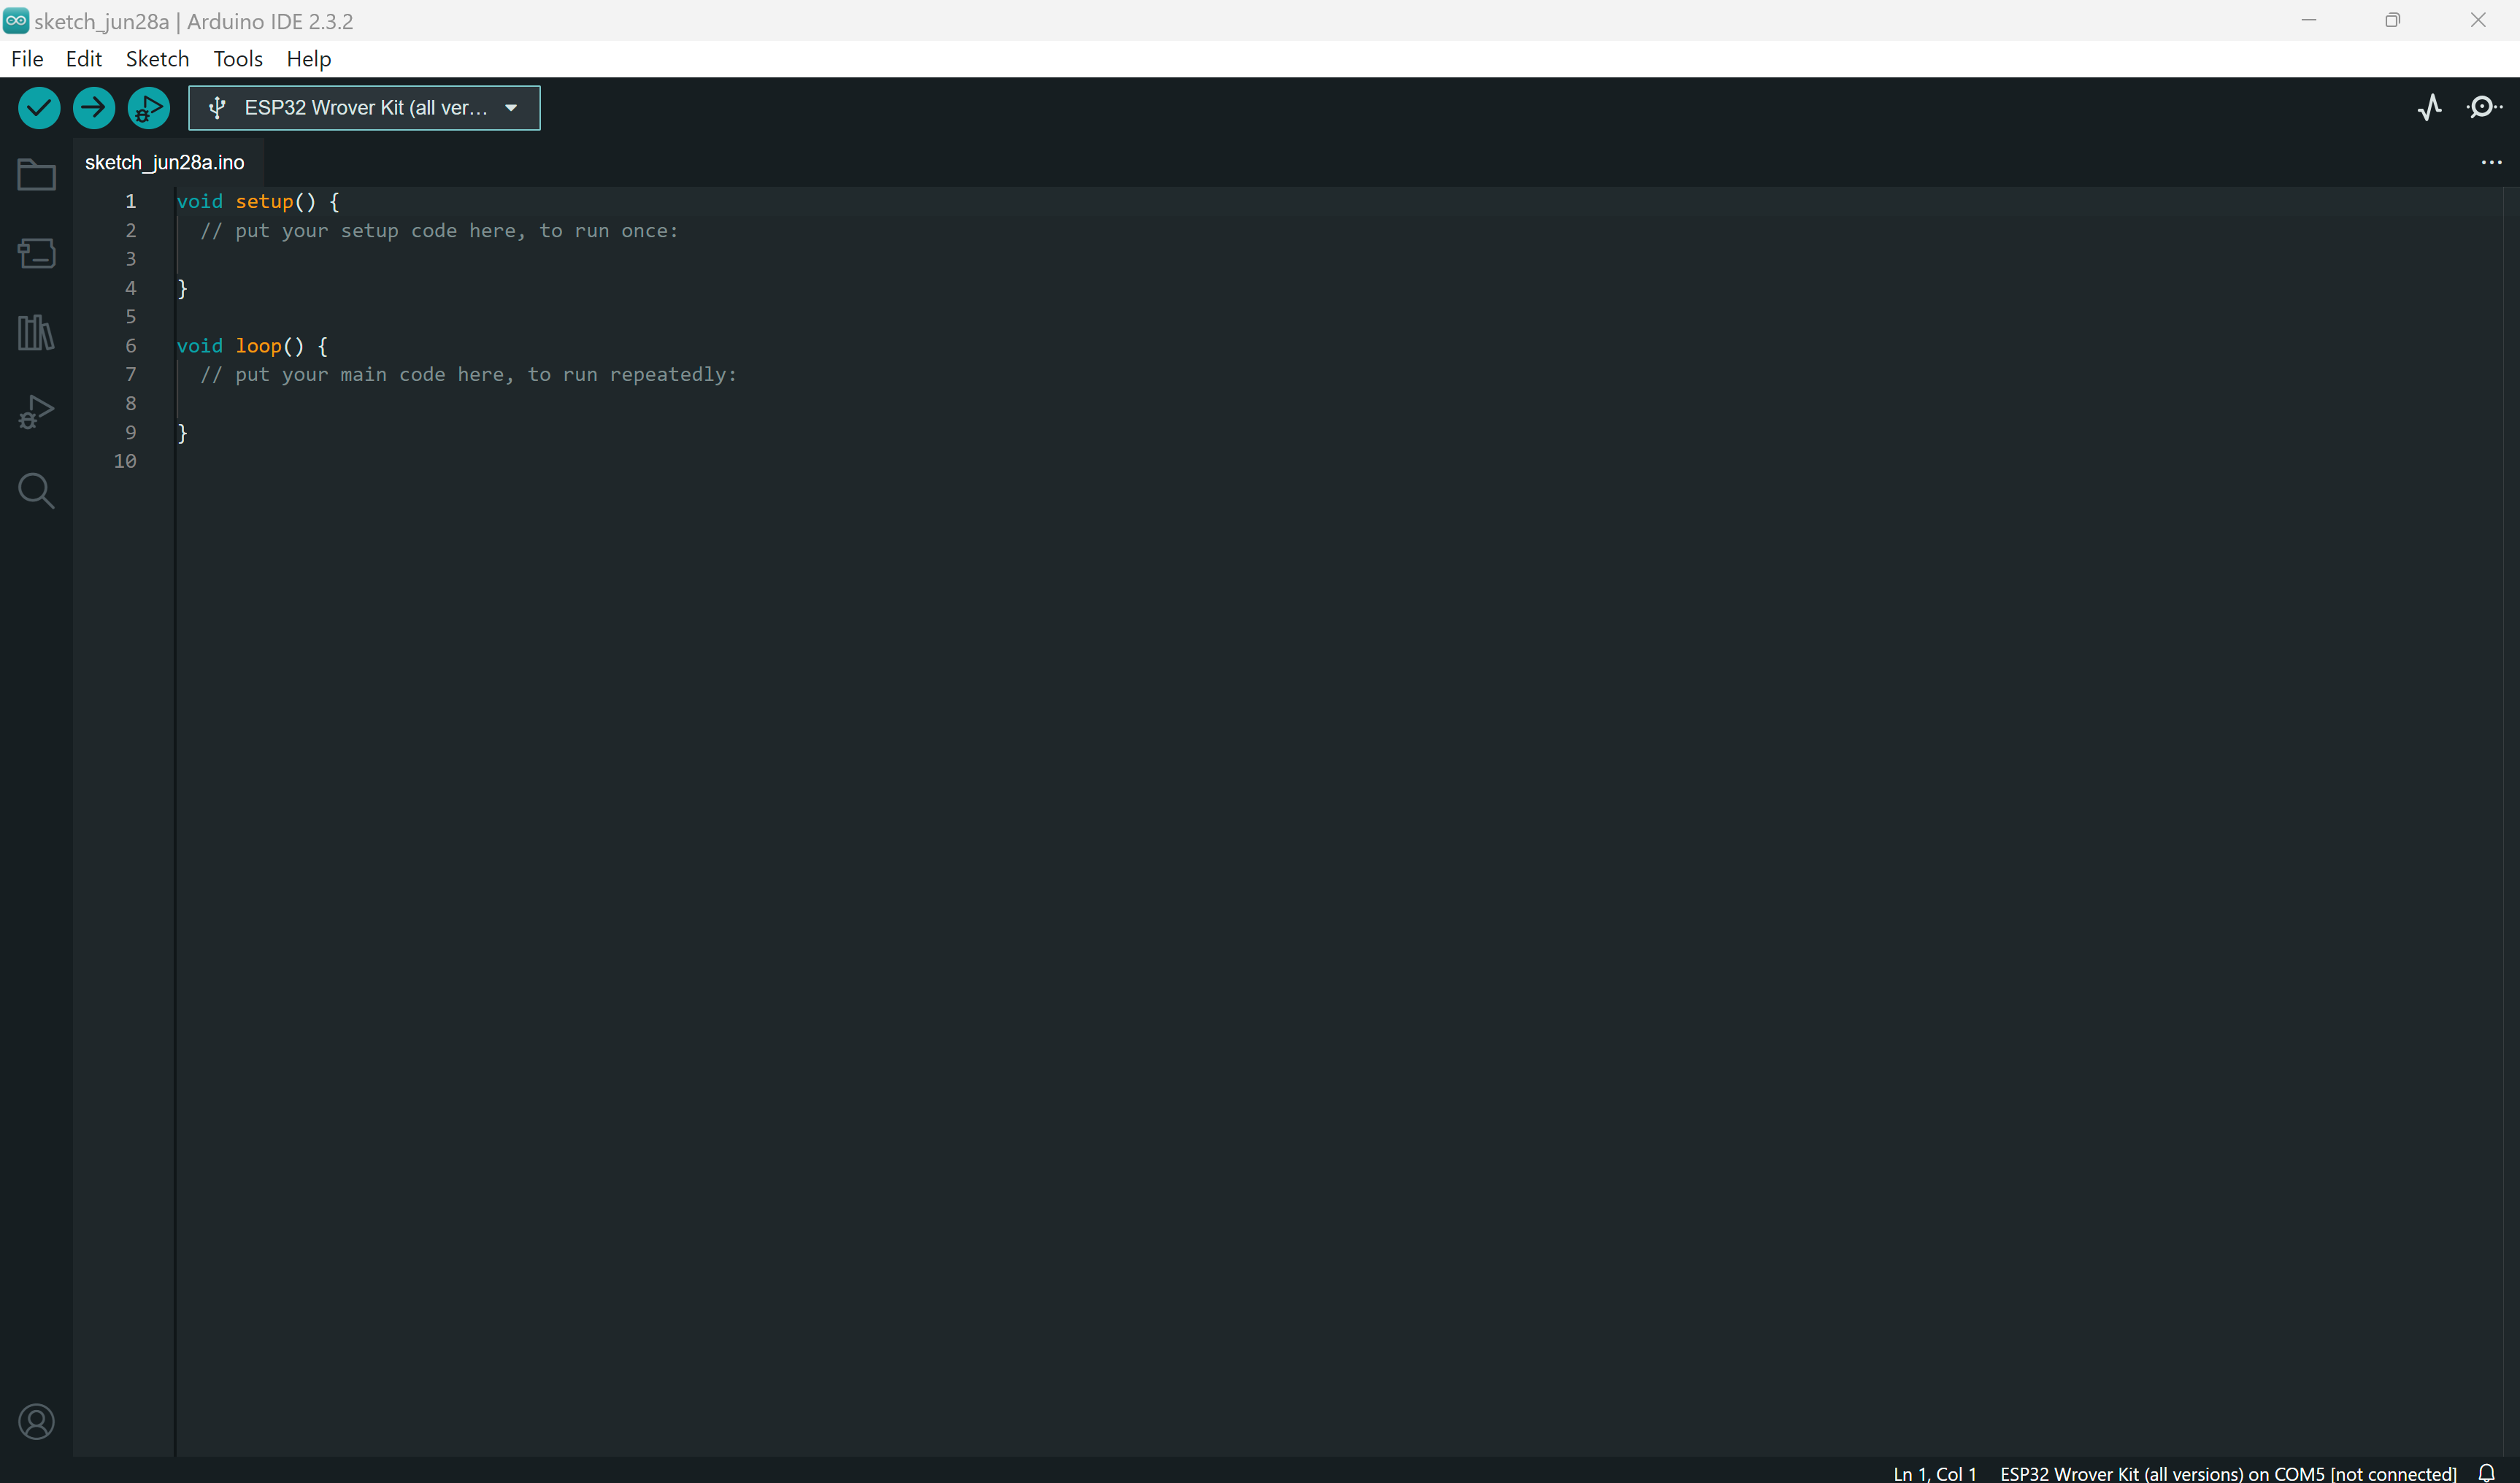
\includegraphics[width=\textwidth]{fig/fig23.png}
		\caption{Arduino IDE}
	\end{figure}
	\item Forbind dit Arduino board til din computer ved hjælp af et USB-kabel.
	\item I Arduino IDE, gå til \textit{Tools} menuen, vælg \textit{Board} og vælg det board, du bruger (f.eks. Arduino Uno).
	\item Gå derefter til \textit{Tools} menuen igen, vælg \textit{Port} og vælg den port, der svarer til dit tilsluttede Arduino board.
\end{enumerate}

\subsection{Oprettelse af et nyt projekt}
\begin{enumerate}[resume]
	\item Klik på \textit{File} menuen og vælg \textit{New} for at oprette et nyt projekt.
	\item Skriv din kode i editoren. Her er et simpelt eksempel:
	\begin{lstlisting}[language=C++]
		void setup() {
			// initialize digital pin LED_BUILTIN as an 
			//output.
			pinMode(LED_BUILTIN, OUTPUT);
		}
		
		void loop() {
			// turn the LED on (HIGH is the voltage level)
			digitalWrite(LED_BUILTIN, HIGH);
			// wait for a second
			delay(1000);
			// turn the LED off by making the voltage LOW
			digitalWrite(LED_BUILTIN, LOW);
			// wait for a second
			delay(1000);
		}
	\end{lstlisting}
	\item Klik på \textit{Upload} knappen (pilen) for at kompilere og uploade koden til dit Arduino board.
\end{enumerate}